%% 
%% ACS project dissertation template. 
%% 
%% Currently designed for printing two-sided, but if you prefer to 
%% print single-sided just remove ",twoside,openright" from the 
%% \documentclass[] line below. 
%%
%%
%%   SMH, May 2010. 


\documentclass[a4paper,12pt,twoside,openright]{report}


%%
%% EDIT THE BELOW TO CUSTOMIZE
%%

\def\dissertationtitle{x86 Semantics in Sail}
\def\wordcount{$11\,838$}

%\usepackage[dvips]{epsfig,graphics} 
\usepackage{epsfig,graphicx,verbatim,parskip,tabularx,setspace,xspace}
\usepackage[svgnames]{xcolor}
\usepackage{listings}
\usepackage[hidelinks]{hyperref}
\usepackage{trfrac}
\usepackage{multicol}
\usepackage{graphicx,grffile}
\usepackage[outdir=./]{epstopdf} % https://tex.stackexchange.com/questions/76455/converted-xxx-eps-converted-to-pdf-not-found
\usepackage{pdfpages}

% https://www.tug.org/FontCatalogue/beramono/
\usepackage[scaled=0.82]{beramono}
\usepackage[T1]{fontenc}

\lstset{
  basicstyle=\ttfamily\small,
  columns=fullflexible,
  breaklines=true,
  postbreak=\mbox{\textcolor{red}{$\hookrightarrow$}\space},
}

\lstdefinelanguage{sail}
  { morekeywords={val,function,mapping,cast,type,forall,overload,operator,enum,union,undefined,exit,and,assert,sizeof,
      scattered,register,inc,dec,if,then,else,effect,let,as,@,in,end,Type,Int,Order,match,clause,struct,
      foreach,from,to,by,infix,infixl,infixr,bitfield,default,try,catch,throw,constraint},
    keywordstyle={\bf\ttfamily\color{blue}},
    morestring=[b]",
    stringstyle={\ttfamily\color{red}},
    morecomment=[l][\itshape\color{DarkGreen}]{//},
    morecomment=[s][\itshape\color{DarkGreen}]{/*}{*/},
    deletestring=[bd]{'},
    escapechar=\#,
    emphstyle={\it},
    literate=
      {\{|}{{$\{|$}}1
      {|\}}{{$|\}$}}1
  }


% https://app.uio.no/ifi/texcount/faq.html#newgroup
%TC:envir lstlisting 1 text
%TC:envir table 0 text
%TC:envir tabular 1 text
%TC:envir figure 0 text

\bibliographystyle{ieeetran}

%% START OF DOCUMENT
\begin{document}

\pagestyle{empty}
\singlespacing
%% 
%% ACS project dissertation template. 
%% 
%% Currently designed for printing two-sided, but if you prefer to 
%% print single-sided just remove ",twoside,openright" from the 
%% \documentclass[] line below. 
%%
%%
%%   SMH, May 2010. 


%%
%% EDIT THE BELOW TO CUSTOMIZE
%%

\def\authorname{Patrick J.\ H.\ Taylor\xspace}
\def\authorcollege{Gonville and Caius College\xspace}
\def\dissertationtitle{x86 Semantics in Sail}

%% FRONTMATTER (TITLE PAGE, DECLARATION, ACKNOWLEDGEMENTS) 
\pagestyle{empty}
\singlespacing
% title page information
\begin{titlepage} 

\begin{center}
\noindent
\huge
\dissertationtitle \\
\vspace*{\stretch{1}}
\end{center}

\begin{center}
\noindent
\huge
\authorname \\
\Large
\authorcollege      \\[24pt]
%\begin{figure}

\includegraphics{CUni3.pdf}
%\end{figure}
\end{center}

\vspace{24pt} 

\begin{center}
\noindent
\large
{\it A dissertation submitted to the University of Cambridge \\ 
in partial fulfilment of the requirements for the degree of \\ 
Computer Science Tripos, Part III} 
\vspace*{\stretch{1}}
\end{center}

\begin{center}
\noindent
University of Cambridge \\
Computer Laboratory     \\
William Gates Building  \\
15 JJ Thomson Avenue    \\
Cambridge CB3 0FD       \\
{\sc United Kingdom}    \\
\end{center}

\begin{center}
\noindent
\today
\end{center}

\end{titlepage} 

% \newpage
% \vspace*{\fill}

\onehalfspacing
\newpage
{\Huge \bf Declaration}

\vspace{24pt} 

I, \authorname of \authorcollege , being a candidate for Computer Science Tripos, Part III, hereby declare that this report and the work described in it are my own work, unaided except as may be specified below, and that the report does not contain material that has already been used to any substantial extent for a comparable purpose.

\vspace{60pt}
\textbf{Signed}: Patrick Taylor

\vspace{12pt}
\textbf{Date}: 02.06.2020


\vfill

This dissertation is copyright \copyright 2020 \authorname. 
\\
All trademarks used in this dissertation are hereby acknowledged.

\newpage

{\Huge \bf Acknowledgements}

\vspace{24pt}

I would like to thank the following people for their contributions to this project.

My supervisors, Prof.~Peter Sewell, Dr Alasdair Armstrong and Dr Robert Norton-Wright, whose suggestions and guidance in the use of Sail made this project possible.

Prof.~Peter Sewell, Dr Alasdair Armstrong and my father for reading through multiple revisions of the dissertation and providing such detailed and insightful comments.

Dr Shilpi Goel who kindly spent the time to respond in great detail to my emails enquiring about her work.

Finally, my parents for the wisdom they impart and to my friends, both in college and CUHWC.

\vspace*{\fill}



\pagenumbering{roman}
\setcounter{page}{0}
\pagestyle{plain}
\tableofcontents
\listoffigures

\onehalfspacing

%% START OF MAIN TEXT 

\chapter{Introduction}
\pagenumbering{arabic} 
\setcounter{page}{1} 

Formal models of instruction set architectures (ISAs) are becoming more prevalent in industry and research.  One model, developed by Shilpi Goel~\cite{goel-thesis}, uses the interactive theorem prover ACL2 and is written in a subset of Lisp.  It models the behaviour and decoding of a large number of instructions from the x86 architecture and provides a base for simulation and formal verification.  In this project I developed a program to translate this ACL2 model into Sail, a language designed by Armstrong et al.~\cite{sail-paper} to model ISA semantics.  The contributions are as follows:

\begin{itemize}
	\item A translation into Sail of all instructions implemented in the original model (excluding floating-point, some system level and some non-deterministic instructions) and the relevant decoding and dispatch routines.
	\item A program to perform this translation and thus handle future development in ACL2.
	\item Validation of the translated model against the original model to give confidence in its correctness.
	\item The discovery of an error in the original model.
  \item Assessment of the coverage provided by a previously-published test suite using the translated model and Sail's coverage tools.
  \item Details of techniques used when performing source-to-source compilation with Lisp as the input language.
\end{itemize}

The rest of this dissertation is structured as follows.  Chapter~\ref{chapter-background} provides the necessary background in the x86-64 ISA, ISA models, Lisp, ACL2 and Sail.  Chapter~\ref{chapter-method} describes the implementation of the translator, focussing on interesting problems that were encountered.  Chapter~\ref{chapter-results} details the methodology in validating the translated model and assessing the test suite and presents and discusses the results.  Chapter~\ref{chapter-related} describes other work and relates it to this project.  Finally, Chapter~\ref{chapter-conclusion} concludes.

For clarity:

\begin{itemize}
  \item The original ACL2 model can be found at: \url{http://www.cs.utexas.edu/users/moore/acl2/manuals/current/manual/index-seo.php/X86ISA____INTRODUCTION}
  \item My Python translator code and the Sail code it generates are attached in the submission.
\end{itemize}


\hypertarget{chapter-background}{
\chapter{Background}\label{chapter-background}}

This chapter covers the relevant background material.  It starts with an overview of ISA models; it then describes the purpose of ACL2, the syntax of Lisp and the ACL2 x86 model, and gives a brief description of some important parts of the x86 ISA.  Finally it presents an overview of Sail and the reasons for wanting to translate the ACL2 model into Sail.

\section{ISAs and ISA Models}

Instruction Set Architectures form the link between hardware and software.  They define how a processor behaves by specifying the number and type of registers, the format of binary instructions, and how executing each instruction affects the state of the processor and memory.  They do not specify the exact hardware implementation, so \emph{microarchitectural} features (such as cache sizes, pipeline depth, superscalar degree and other optimisations) can be tuned to meet performance goals such as performance, price and energy consumption.  ISAs are thus the standard against which processor implementations are verified and the means by which programmers (or rather, compiler writers) know how their software will behave.

However, current specifications for instruction set architectures exhibit a number of problems.  ISA specifications are large: the specification for \emph{Intel 64}, for example, is over 5000 pages long~\cite{background-intel-manual}.  They are also written predominantly in natural language, where the effects of each instruction on the processor state and memory are described in prose.  This results in difficulties for all parties who use such specifications: development of the spec is hard because the effects of changes are unclear; it is difficult to ensure that hardware implementations are compliant; it is difficult to ensure that machine code programs will behave as expected; and their use relies on \emph{a posteriori} knowledge derived, not from the spec, but from experience and observation of previous implementations.

Thus, formal models have started to make an appearance as they significantly reduce the problems above.  One such effort is Arm's Architecture Specification Language (ASL).  Although originally an informal pseudocode-like language, an initiative in Arm, with Alastair Reid as a prominent figure, turned it into a specified executable language~\cite{background-asl}.  Formal models allow design processes and complexity to be managed by running regression tests to gain confidence an implementation matches the specification or proving properties~\cite{background-comp-arch-paper2} about the specification.  Section~\ref{sail-as-target} describes related work on translating ASL into Sail and explains why translating ACL2 into Sail is a significantly harder process.

\section{ACL2 and LISP}

`A Computational Logic for Applicative Common Lisp' (ACL2) comprises a logic, in which users can create models of digital systems, and an interactive theorem prover to prove properties about such models~\cite{background-acl2-homepage}.  The logic in question is an \emph{applicative} subset of Common Lisp---applicative meaning that basic syntax elements (such as lists, arithmetic and conditional operations) are formalised whilst non-functional features (such as objects and circular structures) are not~\cite{background-walking-tour-lisp}.  Whilst the logical side of ACL2 formalises Lisp to allow theorem proving, the use of Lisp itself allows the execution of models as well.

ACL2 is used in industry.  Hunt et al.~describe~\cite{background-ACL2-2017} some notable early projects including the modelling and verifying of a digital signal processor at Motorola and the verification of floating-point division pseudocode at AMD.  Other companies such as IBM and Rockwell Collins also started using ACL2.  The most relevant industrial use is at Centaur Technology, where ACL2 is used throughout the extensive formal verification efforts of Goel et al.~\cite{background-ACL2-2020}.  The x86 ISA model, discussed in the next section, is used as their reference model.

\section{The ACL2 x86 Model}

The ACL2 x86 ISA model~\cite{background-model-homepage} makes use of both logical reasoning and execution: one can prove properties about the model symbolically and formally verify programs against a specification; or, given a memory image including a sequence of x86 instructions and a starting state for the registers, one can emulate its behaviour.  Examples can be found in Goel's original thesis on the model~\cite{goel-thesis}.  The ability to execute instructions is not only useful for simulating programs, but vital for validating the model is correct in the first place.  Without this, reliance would be needed on the human ability to translate correctly the specifications into the Lisp model---a situation antithetical to the original purpose of the model.  Validation of the Sail translation against the ACL2 model is explored in Chapter~\ref{chapter-results}.

The ACL2 implementation models the instruction semantics for many instructions including $218 / 256$ one-byte opcodes and $113 / 256$ two-byte opcodes.

It also models instruction decoding.  This is worth mentioning because x86 decoding is very complex.  Another notable x86 model, developed in the K Framework by Dasgupta et al., does not model decoding at all~\cite[Introduction footnote]{k-framework}, instead opting to call semantic functions based on the assembly code rather than the compiled binary.  Encoded x86 binary instructions may include, amongst others, the following parts:

\begin{itemize}
	\item 0-4 bytes of optional \emph{legacy} prefixes which affect the instruction behaviour (for example, repeating the instruction a certain number of times).  At most one prefix from each of four groups actually affects the behaviour, although more than one from each group may be present in the instruction---in this case, the behaviour is undefined but, empirically, Goel notes, only the last prefix in each group seems to take effect.
	\item An optional \emph{REX} prefix byte for certain instructions.
	\item 1-3 bytes of instruction opcode.
	\item Other instruction-dependant or optional bytes such as \emph{modR/M}, \emph{SIB} and operands, each of which has its own complex semantics.
\end{itemize}

As well as modelling instruction semantics and decoding, the model implements both \emph{application} and \emph{system} level \emph{views}, broadly corresponding to x86 protection rings, but with added utilities in the application-level view to provide functionality expected of an operating system.

It is worth presenting a call trace for an example instruction run under the ACL2 model.  Figure~\ref{diagram-trace} shows the main functions involved in executing the instruction \texttt{add \$0x1,\%eax} (incrementing the value in register \texttt{eax}).  Execution begins at the top-level step function where some decoding occurs.  Once the opcode is found, control is passed, via the one-byte dispatch table, to the \emph{operation specification function} which performs more decoding and finds the operand values, and then to the \emph{instruction specification function} which performs the calculation on the operands, before the results are written back to memory and registers.  The boxes on the right show that this is just one possible execution trace: not only do other instructions exist in the one-byte opcode table, but whole other dispatch tables exist.

Furthermore, functionality such as finding the prefixes of an instruction is difficult in itself and, although only mentioned in the diagram, has a whole call trace unto itself.  This particular example (finding the prefixes) is difficult for two reasons:

\begin{enumerate}
  \item Finding the prefixes is a non-trivial task: some complications were explained above.
  \item Even just reading from memory is a complex task.  For example, multiple levels of address calculation must be performed to go from the \emph{effective} address, through \emph{linear} and \emph{logical} address before the final \emph{physical} address is found.
\end{enumerate}

\begin{figure}
\centering

  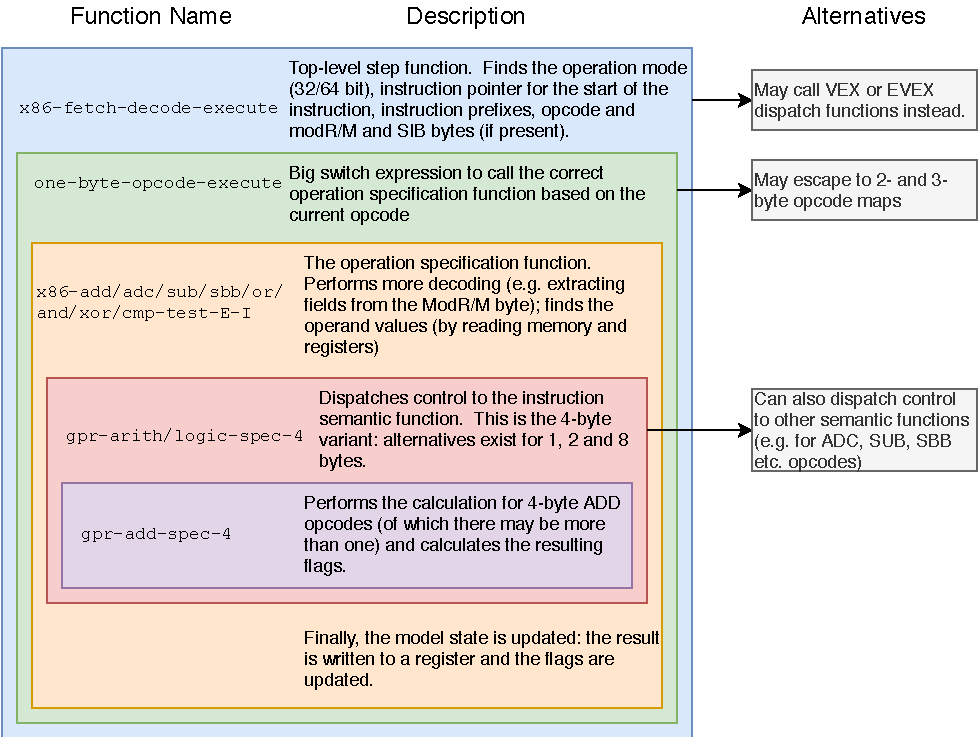
\includegraphics[width=\columnwidth]{../diagrams/trace.pdf}

\caption{Example Call Trace in the ACL2 Model for Instruction \texttt{add \$0x1, \%eax}}
\label{diagram-trace}
\end{figure}

The model itself is spread across $80$ files, of which $41$ represent instruction semantic functions and the rest are the surrounding framework for handling memory, decoding, dispatch and state representation.  This totals over $40\,000$ lines of code, excluding blank lines and comments~\cite[Sec.~3.2]{goel-thesis}

\section{Sail}

Sail is a first-order imperative programming language designed by Armstrong et al.~\cite{sail-paper} specifically for modelling ISAs.  Registers and memory are represented by global state and reads and writes are tracked through the Sail specification with an effects system.  It is statically and strongly typed with a light-weight dependent type system, allowing one easily to write functions which can operate on different data widths.

Like the ACL2 and K Framework models, Sail supports both reasoning and execution however, instead of doing so internally, it generates code for well-known existing systems.  It targets OCaml and C for generating executable emulators and Isabelle/HOL, HOL4, Coq and SMT for logical reasoning.

Sail is also designed to be simple and similar to pseudocode languages used in existing specifications to provide familiarity to engineers, as opposed to ACL2 which has a high entry barrier and a steep learning curve.

\section{Conclusion---Background}

In this chapter we have: noted that ISA models are becoming increasingly important; seen two languages for ISA specification; introduced the ACL2 x86 ISA model; and made the case for translating it into Sail.

Further specific details of Lisp, ACL2, the ACL2 model and the x86 architecture are introduced as they are needed throughout this dissertation.

\hypertarget{chapter-method}{
\chapter{Method}\label{chapter-method}}

This section first describes the method used to translate Lisp to Sail, including an extended example, before going into detail on particular points of interest.  Specifically, we first look at how we can extract type information from Lisp code and fill in the gaps where information is missing.  Next we examine the problems encountered when trying to convert certain pieces of Lisp syntax which may map to more than one piece of Sail syntax and how to disambiguate the available options.  Finally, a brief description of macro handling is given.

\section{Overview}

In a general compiler pipeline, the first stages are lexing a string of characters into tokens before parsing a list of these tokens into an Abstract Syntax Tree (AST).  Fortunately, Lisp's use of prefix (Polish) notation makes it simple to both lex and parse.  For the reader unfamiliar with Lisp, the key feature is that code is represented by lists which are always delimited by brackets.  For instance, the arithmetic expression \[ 1 + (2 \times 3) \] can be represented as the following Lisp expression:

\begin{lstlisting}[language=lisp]
(+ 1 (* 2 3))
\end{lstlisting}

Note that the functions being applied (addition and multiplication) are the first elements in their respective lists and the arguments to which they are applied come after.

Once a Lisp AST has been constructed, it must be translated into a Sail AST.  This is hard, partly due to the complexity of higher-level Lisp forms, and partly because of the desirable properties for the translator.  Specifically, it was decided that the translator ought to satisfy the following properties:

\begin{itemize}
	\item It should be predominantly automatic---it should be able to translate Lisp code to Sail with little manual intervention.
	\item It should produce idiomatic Sail code.
\end{itemize}

In reality there is a trade-off between the two.  At one extreme a completely manual translation would produce highly readable Sail but any change in the ACL2 must also be tracked manually.  At the other end, it would likely be possible to implement a Lisp interpreter within Sail using the lowest level Lisp forms possible (it is possible to construct a Lisp with very few primitives~\cite{lisp-primitives}) but this would be far less readable.  The more realistic, middle-ground, design decisions are which high level functions to translate manually and which to leave to the translator.  For example, the \texttt{rotate-left} function, in ACL2, splits its integer input into two by performing appropriate bitwise mask operations, shifts the two parts into their new positions before \texttt{OR}ing them together.  It would be eminently possible to translate these operations into Sail, but a more idiomatic approach would be as follows:

\begin{minipage}{\linewidth}
\begin{lstlisting}[language=sail]
xl = get_slice_int(placesMod, x, 0);
xh = get_slice_int(width, x, placesMod);
unsigned(xl @ xh)
\end{lstlisting}
\end{minipage}

The \texttt{get\_slice\_int} functions split the input integer, \texttt{x}, into high and low parts, \texttt{xh} and \texttt{xl} respectively, before simply concatenating the results using \texttt{xl @ xh}.  This is far more concise and readable but the implementation required manual inspection.  For this function such effort can be justified as it is a low-level utility function which is unlikely to change.

The previous example was contrived: realistic translation contains far more subtlety.  Examples of why this is the case are detailed in the following sections; however to gain an intuition of the overarching translation technique, an extended example is presented.

\hypertarget{extended-example}{
\section{Extended Example}\label{extended-example}}

This section examines the function in Figure~\ref{bitcount8} which is written in ACL2 and which is part of the x86 model.  Its features are explained as needed, but at a high level, the function counts the number of set bits in an 8-bit unsigned integer.  Further details about many topics introduced in this section, such as macros and typing, are covered in more detail later.

\begin{figure}
\begin{lstlisting}[language=lisp]
(define bitcount8
  ((x :type (unsigned-byte 8)))
  :measure (integer-length x)
  :inline t
  :no-function t
  :verify-guards nil
  :enabled t
  (if (zp x)
      0
    (+ (the (unsigned-byte 1)
         (mbe :logic
              (loghead 1 x)
              :exec  (logand 1 x)))
       (the (integer 0 8)
         (bitcount8
          (the (unsigned-byte 8)
            (mbe :logic
                 (logtail 1 x)
                 :exec  (ash x -1)))))))
\end{lstlisting}
\caption{Example of an ACL2 Function}
\label{bitcount8}
\end{figure}

We proceed by examining each token in the code in turn and explaining how it is handled by the translator.

\bigskip
\begin{lstlisting}[language=lisp]
define
\end{lstlisting}

As mentioned earlier, the first token in a list is the function (or macro) name; the remainder of the list is data it consumes.  Thus, \texttt{define} tells us how to handle the rest of the example, in this case, defining a function.  The question is, how does the translator know what to do with \texttt{define}?  It is convenient to separate into categories the types of symbol the translator might encounter:

\begin{itemize}
	\item Handwritten functions, such as \texttt{rotate-left} above.  When the translator encounters \texttt{rotate-left}, the resulting Sail code is simply a call to the handwritten Sail function \texttt{rotate\_left}.
	\item Previously translated functions.  A function which has already been translated can be translated as a call to that translated function in Sail.  For instance here, \texttt{bitcount8} is used within the \texttt{bitcount8} function (making it recursive).
	\item Special tokens.  It is expedient to handle certain keywords manually.  It is into this category that \texttt{define} falls.  Many such keywords are implemented in Lisp with more primitive constructs (\texttt{define}, for instance, is actually a macro) but we choose to handle them manually for convenience.  Others are primitives for which we have no choice but to handle them manually (e.g.~the token~\texttt{if}).
\end{itemize}

Information about handwritten and previously encountered functions, and special tokens is carried around in an \emph{environment} which is threaded through the translation code.

\bigskip
\begin{lstlisting}[language=lisp]
bitcount8 ((x :type (unsigned-byte 8)))
\end{lstlisting}

The special token translation for the \texttt{define} keyword specifies that the next two Lisp \emph{forms} are the function name and formal parameters respectively.  The fact that a function called \texttt{bitcount8} exists with a bound variable \texttt{x} is thus registered with the environment so that they are available for use when the function body is translated.  Note that the code which translates a form beginning \texttt{define} must handle the list starting with \texttt{x} appropriately: the \texttt{x} is not a function call but the name of the formal parameter.  We also see an example of gaining type information: \texttt{:type} introduces the declaration that \texttt{x} is an unsigned number at most eight bits long (not eight bytes long, confusingly).

\bigskip
\begin{minipage}{\linewidth}
\begin{lstlisting}[language=lisp]
:measure (integer-length x)
...
:enabled t
\end{lstlisting}
\end{minipage}

These \emph{keyword} parameters are used by \texttt{define} and provide instructions to ACL2---in this case they can all be ignored as they do not contribute to the translation.

\bigskip
\begin{lstlisting}[language=lisp]
(if ...)
\end{lstlisting}

The final form in a \texttt{define} is known to be the function body.  We now encounter, again, a list representing some code and so can call the translator function recursively on it.  It finds that, as mentioned above, the handling of \texttt{if} is defined as a special token, and that its structure is \texttt{(if <predicate> <then-branch> <else-branch>)}.

\bigskip
\begin{lstlisting}[language=lisp]
(zp x)
\end{lstlisting}

The first form within \texttt{if} is the conditional predicate.  Once again, the translator is called recursively and finds that zp translates to a function which tests for zero.

\bigskip
\bigskip
\bigskip
\bigskip
\begin{lstlisting}[language=lisp]
0
\end{lstlisting}

The second form is the \texttt{then} branch.  Here the translator must be able to handle number literals.  In general, it must also handle other types of literal as well as some macros which translate as literals.  Fortunately, these are syntactically disambiguated.

\bigskip
% \begin{minipage}{\linewidth}
\begin{lstlisting}[language=lisp]
    (+ (the (unsigned-byte 1)
             (mbe :logic
                  (loghead 1 x)
                  :exec  (logand 1 x)))
           (the (integer 0 8)
             (bitcount8
              (the (unsigned-byte 8)
                (mbe :logic
                     (logtail 1 x)
                     :exec  (ash x -1)))))
\end{lstlisting}
% \end{minipage}

Again, the translator is called recursively on the subsequent nested forms in the \texttt{else} branch.  The tokens \texttt{+}, \texttt{the}, \texttt{unsigned-byte}, \texttt{loghead}, \texttt{integer} and \texttt{logtail} are translated as special tokens or handwritten functions as explained above.  There are three items which do deserve comment:

\begin{enumerate}
	\item \texttt{mbe} is used in the ACL2 code to allow the use of different forms depending on whether the model is being used for logical reasoning or execution (the two forms must be proved to be equivalent).  No such distinction is made in Sail, and so we can pick just one `branch' to translate---here, the calls to \texttt{logand} and \texttt{ash} may be ignored because the \texttt{:logic} branches are chosen.
	\item The call to \texttt{bitcount8} is recursive.  This requires that, when translating \texttt{define}, the presence of the \texttt{bitcount8} function is registered with the environment before the translation of its body.  It can also complicate typing, although here the type can be resolved by the base case in the other branch of the \texttt{if}.
	\item The use of \texttt{x}, the formal parameter to the function also requires its presence to be registered with the environment in a list of currently bound variables.
\end{enumerate}

The translation of the \texttt{bitcount8} into Sail is shown in Figure~\ref{bitcount8-sail}.

\begin{figure}
\begin{lstlisting}[language=sail]
val bitcount8 : (int) -> int effect {escape}
function bitcount8 (x) =
  if (x) == (0)
  then 0
  else (the_range(0, 1, loghead(1, x))) + 
       (the_range(0, 8, bitcount8(
          the_range(0, 255, logtail(1, x)))))
\end{lstlisting}
\caption{Function Shown in Figure~\ref{bitcount8} Translated into Sail}
\label{bitcount8-sail}
\end{figure}

\hypertarget{translator-structure}{
\section{Translator Structure}\label{translator-structure}}

We now describe the structure of the translator from a high level---Figure~\ref{diagram-structure} shows the control flow with the most common paths highlighted in blue and recursion indicated by dotted lines.  Mostly, after a Lisp file has been lexed and parsed, the translator recursively translates code lists (either as special tokens, handwritten functions or functions automatically translated already), as demonstrated in Section~\ref{extended-example}.  Sometimes manual intervention is required to handle very specific cases and, of course, there are base cases such as number literals and strings.  Other patterns (such as how to represent consecutive function definitions) do exist but are uninteresting and elided from the diagram.

\begin{figure}
\centering

  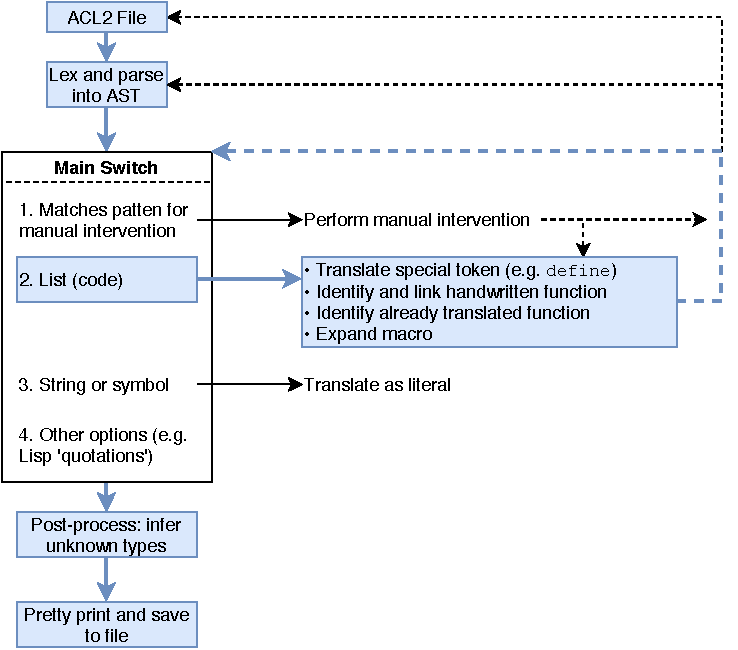
\includegraphics[width=\columnwidth]{../diagrams/structure}

\caption{Translator Structure}
\label{diagram-structure}
\end{figure}

The translator itself (excluding test harnesses) is implemented across $11$ Python files totalling over $7000$ lines.  The largest file implements the special token translation.

Translations of $69$ special tokens have been implemented.  Some of these are one-line functions (such as the translation of \texttt{(in-package ...)}), but most are more lengthy, and some are very complex.  Complicated functions include the translations of: function definitions (\texttt{(define <args> <body>)}), which require careful handling of bound variables, typing, keywords and recursion; and sophisticated local bindings such as the \texttt{b*} form.

Furthermore, there are $74$ support functions handwritten directly in Sail to manage register and memory access and basic bitwise operations.

There are also $15$ more specific manual interventions which capture edge cases.  Creating the patterns on which to select the correct AST elements was sometimes a complex and involved task.  It was also necessary to support both pre- and post-translation interventions, adding to the complexity.

These figures give an idea of the scale of the project and show it to be a large undertaking.

Overall, the translator is a recursive function which translates lists based on the first symbol, taking different actions depending on the category into which that symbol falls.

\hypertarget{typing}{
\section{Typing In General}\label{typing}}

The extended example in Section~\ref{extended-example} demonstrated how the translator recursively translates Lisp forms based on manually defined patterns or functions it has already encountered.  Although careful implementation is required when translating terms, things become even harder when considering types.  This section details some of the problems encountered and their solutions.

There are three issues that make handling types difficult:

\begin{enumerate}
	\item Lisp is dynamically typed but Sail is statically typed.
	\item ACL2 has a rich type system causing unexpected problems  when translating Lisp types.
	\item Some literal Lisp terms translate to different ACL2 literals depending on their context.
\end{enumerate}

This section covers the first two issues by explaining basic type inference and type approximations before describing a richer type inference algorithm.  Section~\ref{nil} covers the third issue.

\hypertarget{basic-types}{
\subsection{Basic Type Inference}\label{basic-types}}

In Sail there is a syntactic obligation to specify types of functions in the source code.  For example, in the simple Sail function below, the specification that \texttt{is\_nat} is a function from \texttt{int -> bool} is mandatory.

\begin{minipage}{\linewidth}
\begin{lstlisting}[language=sail]
val is_nat : int -> bool
function is_nat (x) =
  x >= 0
\end{lstlisting}
\end{minipage}

Lisp, on the other hand, is dynamically typed and there is no syntactic obligation to provide type annotations.  However, in order to translate Lisp code, static type inference must be performed.  In particular, it is necessary, for each function, to infer a type for each formal parameter and to infer a return type.

The latter problem is relatively simple: we use unsurprising type inference rules associated with AST elements to infer the return type of each function.  When inconsistencies arise typing fails and an error is produced, for instance, when the branches of a conditional expression have different types.  Usually typing fails in this way when a heuristic fails to `guess' the correct type in the presence of ambiguity.  More information about such heuristics and why we need them is given in Section~\ref{heuristics}.

The remainder of this section (and indeed Sections~\ref{type-approx} and~\ref{type-algo}) covers the harder problem of inferring the types of formal parameters to functions.

To begin, we note that, fortunately, there are often hints within the ACL2 code.  We saw this in the extended example when the \texttt{:type} keyword was used to infer the type of a variable. There are two general ways in which type information can be specified in ACL2:

\begin{enumerate}
	\item \textbf{Guards}.  Guards are the mechanism most akin to types.  In raw Lisp, a function of $n$ formal parameters can be applied to $n$ actual parameters of any type~\cite{types-about-types}.  Guards restrict the domain of functions so that they only accept arguments which satisfy a given formula~\cite{types-guard-intro}.  For instance, the following snippet indicates that the argument \texttt{result-nbits} is a natural number and \texttt{signed-raw-result} is an integer.

\begin{minipage}{\linewidth}
	\begin{lstlisting}[language=lisp]
(define general-of-spec-fn (result-nbits signed-raw-result)
  :guard (and (natp result-nbits)
              (integerp signed-raw-result))
  ...
	\end{lstlisting}
\end{minipage}

	Guards are used both logically---to reason about functions---and in execution---to allow the underlying Lisp implementation to use functions optimised for specific datatypes rather than having to handle any type.

	\item \textbf{Type Specifiers}~\cite{types-type-spec}.  Type specifiers (type-specs) are more ubiquitous, both in their prevalence and in the variety of forms in which they can appear.  For instance, we can give extra information to function definitions using the form \texttt{(declare <type-spec> v1 ... vn)}~\cite{types-declare} or use a similar technique inlined into the code using \texttt{(the <type-spec> <expr>)}~\cite{types-the}.  Type specifiers are primarily used to improve execution speed but are also added to the \emph{guard obligations} for formal reasoning.  As a concrete example, we saw earlier the following form:

  \begin{lstlisting}[language=lisp]
  x :type (unsigned-byte 8)
  \end{lstlisting}

  The type-spec \texttt{unsigned-byte 8} tells us that \texttt{x} is an eight bit number (not an eight byte number).
\end{enumerate}

The above examples already hint at the large number of ways in which types may be specified in ACL2, and it is from this variety that complexity arises.  Each way of specifying types must be caught (there are at least five different ways: guards; using \texttt{:type}; using \texttt{declare}; inline \texttt{the} expressions and \texttt{the} expressions as part of a \texttt{b*} form)~\cite{types-guard-intro,types-xargs,types-declare,types-the,types-b-star}.  Furthermore, different forms suggest different translations: \texttt{declare} and \texttt{the} forms are two contrasting examples.  \texttt{declare} forms give us information about the type of a function and so influence the top-level \texttt{val} declaration in Sail whereas \texttt{the} forms are best translated inline.  An example is presented in the following code snippet.

\begin{minipage}{\linewidth}
\begin{lstlisting}[language=sail]
val the_nat : int -> nat effect {escape}
function the_nat (i) = {
	assert (i >= 0);
	i
}
\end{lstlisting}
\end{minipage}

Here we see that Sail incorporates flow-sensitive typing.  The \texttt{assert} statement provides typing information to the next line: specifically, that \texttt{i >= 0} and hence can be given the type \texttt{nat}.  If, at runtime, \texttt{i < 0} then the \texttt{assert} throws an exception (this requires the \texttt{escape} effect to be declared as described in Section~\ref{effects}).  In this way, translation is made easier but some static type-safety is lost: Sail was designed to allow this trade-off when implementing the ASL to Sail translator~\cite{sail-paper}.

In capturing useful instances of type information we must also be able to translate the guards and type-specs themselves.  Type-specs are relatively straightforward in that their syntax contains a small number of oft-used constructs.  Guards are more complex in that they can, and do, use arbitrary formulae.  They are also less prevalent than type-specs.  Overall, we have the same problem of what to translate manually or what to ignore.

Finally, is it worth noting that we cannot extract all the necessary type information directly.  For instance, consider this following snippet from the start of a function definition:

\begin{minipage}{\linewidth}
\begin{lstlisting}[language=lisp]
(define x86-effective-addr
    ((proc-mode 
        :type (integer 0 #.*num-proc-modes-1*))
     p4
     (temp-RIP
        :type (signed-byte #.*max-linear-address-size*))
  ...
\end{lstlisting}
\end{minipage}

Here, the types of the formal parameters \texttt{proc-mode} and \texttt{temp-rip} are specified using type-specs, but the parameter \texttt{p4} has no type information.  The solution to this problem is described in Section~\ref{type-algo}.

\hypertarget{type-approx}{
\subsection{Type Approximations}\label{type-approx}}

In this section we first see an ACL2 type-spec which suggests a certain translation to Sail.  We then see why this translation actually causes problems and how to mitigate them.

Consider the following ACL2 type-spec applied to an expression, \texttt{x}:

\begin{lstlisting}[language=lisp]
(the (integer i j) x)
\end{lstlisting}

Unsurprisingly, this specifies that \texttt{i <= x} and \texttt{x <= j}.  It is thus very tempting to assign \texttt{x} a \texttt{range} type in Sail, specifically, \texttt{x : range(i, j)}.

Now consider passing \texttt{x} into a basic function which returns the first 64 bits of a number as a natural:

\begin{lstlisting}[language=sail]
(n64 (the (integer i j) x))
\end{lstlisting}

A very tempting type signature for the translation of \texttt{n64} in Sail is:

\begin{minipage}{\linewidth}
\begin{lstlisting}[language=sail]
val n64 : forall 'n 'm.
          (range('n, 'm)) -> range(0, 2^64 - 1)
\end{lstlisting}
\end{minipage}

The assumption is that a range type being passed in, say \texttt{range(i, j)}, will have \texttt{i} and \texttt{j} unified with \texttt{'n} and \texttt{'m}.  This assumption is wrong.

This is because the type signature shown above for \texttt{n64} is internally equivalent to:

\begin{minipage}{\linewidth}
\begin{lstlisting}[language=sail]
val n64 : forall 'n 'm 'c,
          'n <= 'c <= 'm.
          int('c) -> range(0, 2^64 - 1)
\end{lstlisting}
\end{minipage}

Neither \texttt{'n} nor \texttt{'m} appear in the function argument or return type, and so are unconstrained.  Effectively, they could be picked arbitrarily, reducing the type to \texttt{val n64 : int -> range(0, 2\^{}64 - 1)}.  In reality the type checker simply fails as it is unable to instantiate the function type.

For this reason, it is sensible to assume that all numeric argument types are integers (the supertype for all numeric types in Sail~\cite{sail-manual}).  In this case, the type of \texttt{n64} would become:

\begin{lstlisting}[language=sail]
val n64 : int -> int
\end{lstlisting}

It is reasonable to ask why the return type is now \texttt{int} as well.  In general, it is not immediately obvious how to infer the most constrained return type of functions and considering all numeric return types as integers was the expedient solution.  There is the possibility for future work of performing a whole AST transformation after translation has occurred to examine how functions are called and attempt to tighten up the top-level types in Sail.

Likewise, it would also be possible to consider all numeric types as the \texttt{bits('n)} Sail type.  Here we would both be obliged to specify the bit width and would be further from the ACL2 handling of numerics.

Overall, practical type checking is performed at run time using \texttt{assert} statements in the translation of \texttt{the} expressions as demonstrated in Section~\ref{basic-types}.  This is more in line with the programming style of the ACL2 model.

\hypertarget{type-algo}{
\subsection{Richer Type Inference}\label{type-algo}}

We saw in Section~\ref{basic-types} that we can often infer the types of formal parameters to functions from annotations in the ACL2 syntax, but that occasionally the necessary information is missing or hard to extract.  We want to be able to reconstruct this data in order to be able to generate the mandatory type specifications for Sail.  This section first shows some examples and then describes the algorithm developed to do this.

The example where the type of \texttt{p4} is not specified is repeated as follows:

\begin{minipage}{\linewidth}
\begin{lstlisting}
(define x86-effective-addr
    ((proc-mode :type (<type-spec>*))
     p4
     (temp-RIP :type (<type-spec))
	...
\end{lstlisting}
\end{minipage}

Section~\ref{type-approx} showed that any numeric type in ACL2 can be approximated as an integer in Sail, however typing all functions with integers is not a universal solution: bools, strings and option types also exist.

One way of gaining information about \texttt{p4} is to see how \texttt{x86-effective-addr} is used elsewhere in the codebase---specifically, what type is passed in for the actual parameter of \texttt{p4}.  For example, in one of the semantic functions for a MOV instruction, this function is used as follows:

\begin{minipage}{\linewidth}
\begin{lstlisting}
(x86-effective-addr proc-mode p4? temp-rip
                    rex-byte r/m mod sib 0 x86)
\end{lstlisting}
\end{minipage}

Earlier in the same function we find that \texttt{p4?} was calculated using an equality test:

\begin{minipage}{\linewidth}
\begin{lstlisting}[language=lisp]
(b*
	((p4? (equal
          #.*addr-size-override*
          (prefixes->adr prefixes))))
	...)
\end{lstlisting}
\end{minipage}

The function \texttt{equal} (and other equality tests) are functions which are translated manually.  Specifically, we translate \texttt{equal} to the Sail function \texttt{==} which has a return type of \texttt{bool}.  From here we can work our way backwards: \texttt{p4? : bool} means that the \texttt{p4} formal parameter of \texttt{x86-effective-addr} must also have type \texttt{bool}.

We could also have gone in the other direction: examining where \texttt{p4} is used \textbf{within} \texttt{x86-effective-addr}.  In this case, it is only used as the conditional of \texttt{if} expressions.  This agrees with the above conclusion that \texttt{p4} is a boolean.  Do note, however, that we cannot infer a boolean type from use in the conditional of an \texttt{if}.  This may seem counter-intuitive and it is, in fact, symptomatic of a larger problem described in Section~\ref{nil}.

The question now becomes how to generalise this technique.  There are two key insights which help us do this.

Firstly, this problem relates solely to instances of bound variables whose type is unknown.  Although other type ambiguities do arise, as detailed in~\ref{nil}, this problem is decoupled.  These bound variables are generated in a single place: the definition of functions.  The other piece of Sail syntax which generates variables is the \texttt{let} binding, but any variable of unknown type generated here will only inherit an unknown type from a previously bound variable.  We can think of all functions in the translation being built up from primitives: literals, handwritten functions (which have well-specified types) and bound variables.  Thus, resolving the type of a bound variable will have effects elsewhere in the code as the affect percolates upwards.

The second insight is that, instead of thinking about working up or down the AST as in the examples above, we can resolve the type of unknown bound variables using applications of functions to arguments.  For each formal/actual parameter pair we may be able to unify the type of one to the type of the other.  So, the application \[(\lambda \textrm{ \textless formal\textgreater } . \textrm{\textless expr\textgreater} ) \textrm{\textless actual\textgreater}\] gives four situations:

\begin{enumerate}
  \item Formal type unknown, actual type unknown---unification is impossible.
  \item Formal type known, actual type unknown---actual type becomes formal type.  E.g.
  \[ (\lambda (x : \textrm{nat}).e)(x : \textrm{???}) \]
  This case is similar to how type inference algorithms such as Hindley-Milner infer types in the current environment.
  \item Formal type unknown, actual type known---formal type becomes actual type.  E.g.
  \[ (\lambda (x : \textrm{???}) . e) (2 : \textrm{nat}) \]
  This case is not used in type inference algorithms where functions may be polymorphic, but is acceptable here as we assume monomorphism.
  \item Formal type known, actual type known---unification unnecessary.
\end{enumerate}

Note that resolving at applications covers both of the situations in the example above.  When we examine what is passed in as the actual of \texttt{p4} we are working up the AST: this corresponds to an unknown formal but a known actual.  When we look at where \texttt{p4} is used within the function, we proceed downwards, further into the AST.  We hope to find an instance where \texttt{p4} is used as an actual parameter to a function where the corresponding formal has a known type.

This leads us to a fixed point algorithm where we first collect instances of function applications then iteratively resolve instances of bound variables until no changes occur.   At each iteration, the number of unresolved bound variables must either decrease or stay the same.  Hopefully, by the end, all variables of unknown type will be resolved.

There are a few points to note about the implementation:

\begin{itemize}
  \item The algorithm required a mechanism to collect instances of function applications.  In reality, a more general method was implemented to walk an AST and return instances of AST elements satisfying a certain predicate.
  \item Taking an object-oriented approach to representing the Sail AST helped with the resolution process.  When a function is translated it creates an object for each of its formal parameters---a bound variable.  When a variable is used, the same object is referenced.  This removes the need to have a look up table of bound variables and their corresponding types for each function.
  \item Originally the analysis was performed on a per-file level.  Unfortunately, it was necessary to expand this to a global AST analysis to be able to resolve all instances of unknown types.  This is, of course, at the expense of having to translate and store the whole AST before any files are written out.  An alternative would have been to manually intervene when such cases arose, reducing automation.
  \item Once the type of a bound variable has been resolved, its type percolates elsewhere.  The order in which bound variables are resolved will affect performance, however the best order will depend on the AST in question.  For example, a top-level function may have an unknown formal but a known actual, the resolution of which allows the resolution of a function contained therein, and so on for an arbitrary depth.  Here, resolving the top most function first and working down the AST is optimal and results in a time linear in the depth.  Working upwards, however, we would only hit the first resolution having been through all applications, resulting in an overall quadratic time.  On the other hand, working upwards would be optimal if the item that resolves the chain is located at the bottom where an actual is unknown but a formal is known.
\end{itemize}

The overall process can be described in terms of typing rules.  Classically, a typing rule may infer the type of an application from the type of the function and the actual parameter to which it is applied:

\[
\trfrac[(\emph{app})]
  {f : \tau \rightarrow \tau' \qquad
  x : \tau}
  {f x : \tau'}
\]

In the algorithm presented above, we invert the typing rule in two ways:


\begin{multicols}{2}
\[
\trfrac[(\emph{infer-app1})]
  {f x : \tau' \qquad
  f : \tau \rightarrow \tau'}
  {x : \tau}
\]

\[
\trfrac[(\emph{infer-app2})]
  {f x : \tau' \qquad
  x : \tau}
  {f : \tau \rightarrow \tau'}
\]
\end{multicols}

As a final note, the implementation assumes that functions are not polymorphic: the type of each function must be able to be directly represented in terms of concrete types.  This is a reasonable assumption to make in the context of ISA specifications as there is little generic code.

\hypertarget{effects}{
\subsection{Effects and State}\label{effects}}

Another mandatory piece of Sail syntax is the specification of effects.  Effects include reading and writing registers and memory and throwing exceptions.  The effects of each handwritten function must be carefully specified.  This allows for generated functions to calculate their effects: the union of the effects of functions they call.

It is also worth mentioning the difference in state representation between ACL2 and Sail.  ACL2 uses the typically functional style of threading the state through the whole model in the form of an \texttt{x86} parameter for most functions.  Sail specifies registers as global state and interacts with an external memory simulator.  Fortunately, there are a very small number of ACL2 functions which access state---few enough that their types, effects and functionality can all be translated manually.

\subsection{Conclusion---Typing}

In this section we have seen why the translator needs to infer function types from the ACL2 model.  It does this mostly from type annotations in the ACL2 code but analyses the translated AST to fill in the gaps and to infer return types.  We also saw approximations that were made to help interface with the Sail type system.

The next section goes into detail on some terms which have ambiguous translation and how such cases are handled.

\hypertarget{nil}{
\section{Translating \texttt{nil}}\label{nil}}

We have seen that the top-level translation function switches on the first item of a list which represents code---the first item is the function being applied---and recursively translates sub-expressions as necessary.  For the most part, translation is deterministic: there is exactly one course of action to take for each function symbol.

Unfortunately, this is not universally true.  This section details one particular and very prevalent exception, explains the ways in which we handle it and concludes with some brief examples of other anomalies.


\subsection{The Problem with \texttt{nil}}
The most common ambiguous Lisp expression is simply \texttt{nil}.  It is tempting to think we can translate \texttt{nil} simply to the boolean value \texttt{false}.  This is not the case.  Unlike in ClojureScript where Sierram and VanderHart note that it is possible to translate Lisp's \texttt{nil} to JavaScript's \texttt{null}~\cite[ch.~5, p.~42]{clojure-script-nil}, there is no single value to which we can map \texttt{nil}.

Instead, \texttt{nil} is a \emph{falsey} value, and as Staples notes~\cite{staples}, \emph{can} represent \texttt{false} but, depending on context, may need translating as the empty list or \texttt{None()} of the \texttt{option} type.  For those unfamiliar, the \texttt{option} type indicates the presence or absence of a value and has two constructors: \texttt{None()} and \texttt{Some(<value>)}.

In the ACL2 x86 model, the main issues arise in distinguishing between \texttt{false} and \texttt{None()}, instances of which occur throughout the codebase.  For instance, in a specification function for a bitwise shift, we have the form \texttt{(mv 0 nil 0 0)}.  This returns multiple values from a function, one of which is \texttt{nil}.  In this case, as it happens, \texttt{nil} ought to be translated as \texttt{false}, given the other branches the function may take.  On the other hand, we also have instances scattered throughout the codebase of the form \texttt{(mv <symbol> <exprs>)} where the first value returned is a symbol used for error reporting.  If there is no error, we have \texttt{(mv nil <exprs>)}---we choose to translate these errors as expressions of the type \texttt{option(string)}, so here \texttt{nil} ought to be translated as \texttt{None()}.  Clearly it is impossible to distinguish the two cases given just the \texttt{mv} forms (which is all the main translator function sees).

One possible solution would be to translate all instances of \texttt{nil} to \texttt{None()}, not trying to infer its type, then wrap instances where it is used in a boolean context in the function \texttt{is\_some}.  Indeed, \texttt{is\_some} is used, as described later but, in general, such a blanket approach would produce undesirable results as all literals would have to be wrapped in an \texttt{option} type as well.  A more nuanced approach is needed.

\hypertarget{heuristics}{
\subsection{Heuristics}\label{heuristics}}

Although Staples~\cite{staples} does provide some infrastructure for extensible type `guessing', it is not the focus of his paper.  This section, however, details techniques that were used in this project to implement more refined type guessing.

The first heuristic is simple.  As mentioned, we find that the code adheres to an informal discipline where a \texttt{nil} in the pattern \texttt{(mv nil <exprs>)} corresponds to an error of type \texttt{option(string)} being returned in a different branch.  As such, a relatively reliable guess is to translate all instances of \texttt{nil} to \texttt{None() : option(string)} when they appear as the first returned value in an \texttt{mv}.  Indeed, empirically we can extend this to translating all instances to  \texttt{None()} by default and amending them only if we receive information to the contrary based on the alternative schemes below.

The previous heuristic was a blanket `zeroth-order' approach in which we took no account of context.  This next heuristic does consider some basic typing.  We saw in Section~\ref{typing} that we do our best to infer the types of formal parameters to functions.  In some cases, this can help us infer the type of \texttt{nil}.

Specifically, if a function has a formal parameter whose type has been inferred as boolean, then we can translate a \texttt{nil} to which it is applied as \texttt{false : bool}.  A similar method is used when \texttt{nil} is provided as a default value to keyword or \emph{optional} formal parameters~\cite{types-xargs} which have been typed as boolean.

Other first-order cases include:

\begin{itemize}
  \item In some contexts we can infer \texttt{nil} is a boolean.  Examples include instances of the form \texttt{(if <cond> t nil)}, the type-spec \texttt{(or t nil)} and the guard \texttt{booleanp}.  In each case it is highly likely the associated \texttt{nil} can be translated as a boolean.
  \item Sometimes data is stored in array literals.  For example, an array stores \texttt{t} or \texttt{nil} for each opcode depending on whether the \texttt{modR/M} byte should be present in the encoded instruction.  Again, we are fairly safe in translating these values as booleans.
\end{itemize}

Despite these heuristics, manual intervention is sometimes still necessary.  Practically, this is achieved by checking each Lisp form against a list of predicates.  If one of the predicates is satisfied, the form is not passed to the main translation function but instead executes some custom code.  The predicates can be arbitrarily complex and reference any state in the current environment: it is not uncommon to match against the name of the current function being translated in order to implement custom translations.  Some examples can be found in sections~\ref{similar-problems} and~\ref{macros}.

The advantage of this flexibility comes at the cost of over-specialisation: changes in the ACL2 source code could easily cause some interventions to stop working.  There is also the risk of implementing what is effectively the same intervention multiple times without noticing, where a more general rule would work better.

\hypertarget{nil-algo}{
\subsection{A Further Solution}\label{nil-algo}}

In order to try to reduce the number of manual interventions, a more nuanced approach is desirable.  This problem is different from the one we saw in Section~\ref{type-algo}.  In that case, uses of bound variables of unknown type were easily tracked and the point at which types were resolved was clearly at function applications.  As described in the previous section, we do already test for \texttt{nil} being used as a formal parameter in a boolean context.

Instead, we look for a different syntactic structure which will allow us to unify an unknown type for a \texttt{nil} with a known type generated elsewhere in the code.  We alight on conditional expressions.

It is at first tempting to think that we may instantly assign the boolean type to \texttt{nil}s used in the predicate for an \texttt{if} expression.  This, again, is unfortunately not the case: given the falsey nature of \texttt{nil} other types may be used in this context.  Consider a variable \texttt{flg : option(string)} representing a possible error from a function call. A common pattern is to perform the test \texttt{(if flg <expr-involving-flg> <otherwise-expr>)}.  We can handle this situation easily by wrapping expressions of type \texttt{option} in the predicate \texttt{is\_some} when they are supposed to be used in boolean contexts, but cannot infer they are a boolean type just because they are used in such contexts.  This situation is similar to scripting languages such as Python which can use, for example, lists in boolean contexts to check for empty lists.

What we can do is compare the two branches of an \texttt{if} expression (or the multiple branches of \texttt{match}).  This gives us four cases similar to the typing algorithm: if both branches represent \texttt{nil}s or neither is \texttt{nil}, no resolution takes place; whereas if exactly one branch is \texttt{nil} and the other has a well-specified type, we can use that to type the \texttt{nil} branch.

However, whereas in function application, unification inferred the type of exactly one bound variable, the branch of an \texttt{if} expression may represent more than one \texttt{nil} expression.  For example, consider the following contrived example:

\begin{lstlisting}[language=lisp]
(if <cond1> (if <cond2> nil nil) ("Some string"))
\end{lstlisting}

The challenge in this case is to collect the \texttt{nil} terms in the inner \texttt{if} which need unifying.  Cases of this form do appear in the ACL2 model.

It is at this point where the law of diminishing returns comes into effect.  It would certainly be possible to generalise this approach such that information about \texttt{nil}s can be gained an arbitrary number of levels up the AST, with each syntactic element providing different information based on its structure; however with the heuristics and algorithm already described (which considers a single level of condition expression), most cases are handled correctly as it is.

Once again, we can express the concept behind the algorithm by inverting the typing rule for \texttt{if}.  Whereas a classical typing rule may read:

\[
\trfrac[(\emph{if})]
  {b : bool \qquad
  e_1 : \tau \qquad
  e_2 : \tau}
  {\textrm{if } b \textrm{ then } e_1 \textrm{ else } e_2 : \tau}
\]

one of the symmetric inverted versions becomes:

\[
\trfrac[(\emph{infer-if1})]
  {e_1 : \tau}
  {e_2 : \tau}
\]

for $e_1$ and $e_2$ in the expression \[\textrm{if } b \textrm{ then } e_1 \textrm{ else } e_2\]

The main difference between the way in which we type \texttt{nil}s and the way in which we type bound variables can be thought of as the difference between traversing the AST horizontally, in the case of the former, and vertically in the case of the latter.

\hypertarget{similar-problems}{
\subsection{Similar Problems}\label{similar-problems}}

There also exist other Lisp expressions whose translation is ambiguous, although they are far less common:

\begin{itemize}
  \item The symbol \texttt{t} is almost always translated as \texttt{true : bool}, but occasionally must be translated as \texttt{Some(...)}, where we have to come up with the contents.  In reality, these cases are so rare that a manual intervention for each is preferred.
  \item Error reporting has been approximated by using Sail exceptions.  In this case, an inline \texttt{throw} statement in Sail takes on a type appropriate to its context.  The typing algorithm for \texttt{nil} described above is used to infer most instances of \texttt{throw}.
\end{itemize}

\subsection{Conclusion---\texttt{nil}}

This section has shown why the ambiguity of \texttt{nil} makes its translation awkward.  It has also described the heuristics we use to avoid the problem and an algorithm for helping automatic decisions to be made.

\hypertarget{macros}{
\section{Macros}\label{macros}}

Lisp has a very rich macro language which can generate arbitrary Lisp code.  Without embedding a Lisp interpreter within Sail (or dynamically linking to a running ACL2 session) we must expand macros at translate time (at which point we can translate the expanded code) or handle them manually.  Macros are used for code generation extensively throughout the project, so the debate becomes, again, which to expand automatically and which to translate manually.  This section briefly describes some examples.

We frequently find snippets which use \texttt{make-event} as follows:

\begin{minipage}{\linewidth}
\begin{lstlisting}[language=lisp]
(make-event (add-af-spec-gen-fn  8))
(make-event (add-af-spec-gen-fn 16))
(make-event (add-af-spec-gen-fn 32))
(make-event (add-af-spec-gen-fn 64))
\end{lstlisting}
\end{minipage}

This code uses uses the function \texttt{add-af-spec-gen-fn} to generate code specialised for different data widths.  The current solution is to define a special token translation for the macro \texttt{make-event}: a running instance of ACL2 gives us the AST generated by a call to \texttt{add-af-spec-gen-fn}, the result of which we then pass to the function which translates function definitions.  Another possibility is to automatically identify instances of the above pattern and, following the example of Armstrong et al.~\cite[Sec.~3.1]{sail-paper}, leverage Sail's dependent type system.  For example, we could generate a Sail function with the following type signature where the input type depends on the term to which the function is applied:

\begin{minipage}{\linewidth}
\begin{lstlisting}[language=sail]
val add_af_spec : forall 'm,
                  'm in {8, 16, 32, 64}.
                  bits('m) -> bit
\end{lstlisting}
\end{minipage}

However, this would be considerably harder as it would necessitate handling Lisp quasiquotations: we are currently better served by using the underlying Lisp for this instead.

The largest examples of code generation are the dispatch functions which execute the correct semantic function based on the opcode of the current instruction.  These macros expand to many thousands of lines of Sail code.

At a lower level, it is sensible to handle some macros manually.  For example, it turns out that \texttt{OR} is a macro with some subtleties.  In most cases, a translation to the expected function with type \texttt{(bool, bool) -> bool} works perfectly well.  However, in reality, the \texttt{OR} macro expands to a form which returns its first non-\texttt{nil} argument, or \texttt{nil} if all arguments evaluate to \texttt{nil}.  This unusual behaviour is used, but only occasionally, and so a manual intervention in these cases is a good solution.

\section{Conclusion---Method}

This chapter described interesting implementation details and design decisions of the translator and presented two algorithms to enhance type inference.  It started by presenting an extended example and an overview of the translator.  It then went into detail about typing ACL2 code so we have enough information to generate Sail functions, including how we extract basic types, how to fill in the gaps, how \texttt{nil} presents an ambiguity in translation and how to solve the issue.  Finally, a brief description of macro handling was given.

Throughout the chapter we saw examples of two important points.  Firstly, the number of Lisp forms which required special token translation demonstrates the large scale of the project.  Secondly, the number of forms which required a manual intervention to override, generally good, default assumptions also added to the complexity of the project both in debugging where and why the issues arose and in developing correct interventions to solve them.

\hypertarget{chapter-results}{
\chapter{Results}\label{chapter-results}}

The aim of the project was to produce a translator which could automatically convert the x86 ACL2 model to Sail code.  The evaluation of the translator, however, for a large part relies on the artefact it produces: the Sail model itself.  This chapter first describes how the Sail model is validated against the Lisp model then presents and discusses the results of this validation and an evaluation of the test suite used.

\section{Methodology}

This section describes the technique of \emph{co-simulation} and how coverage analysis is used to evaluate the quality of a chosen test suite.

\subsection{Co-simulation}

It is important that we have a high degree of confidence that the semantics of the translated model match those of the original ACL2 model.  One approach, called co-simulation, makes use of the ability to execute the model.  Co-simulation involves running the same series of instructions, from the same starting state, in both models, and comparing the results.  The resolution and detail with which states are compared can vary:

\begin{itemize}
  \item The information logged can include registers and memory reads and writes.  In this project we choose to track only register state.
  \item Logging can occur at the end of a program run, at specific breakpoints or at the end of every cycle.  To  ensure each tested instruction executes correctly we opt for the final approach here.
\end{itemize}

Co-simulation is widely used to validate ISA models against results from real processors and was used in Goel's work~\cite{goel-thesis} to validate the ACL2 model.  Mismatches in states between the model and a processor indicated modelling errors which were corrected.  Here, co-simulation is used to provide confidence that the translation matches the model.  Mismatches mostly indicated translation errors: they were investigated by stepping through pieces of custom assembly code to find the source of the problem before being corrected.  Details of the results are reported in the next section.

In terms of implementation, the ACL2 model was already equipped with instrumentation functions which could log the output needed.  However, some extensive implementation of similar functions at the Sail end and of scripts to compare outputs from the respective models was required.

\hypertarget{methodology-coverage}{
\subsection{Coverage}\label{methodology-coverage}}

It is clearly impossible to exhaustively test every possible input to the model because the state space is too large (the contents of main memory can itself be considered an input).  Thus, we are forced to choose test inputs.  The choice of instructions to run affects the resultant level of confidence that the translation is correct.  For this reason, it is useful to have some idea of instruction \emph{coverage}---a measurement of how much of the model has been tested.

This project used Sail's inbuilt coverage tool, which, for a particular execution run, reports the branches which were taken out of all possible branches in each Sail source file.

\hypertarget{methodology-test-suite}{
\subsection{Test Suites}\label{methodology-test-suite}}

The test programs used in Goel's original co-simulation of the model were chosen `more or less randomly\ldots with judiciously chosen inputs that represent certain classes of possible input values'~\cite{goel-thesis} but were not detailed.  Furthermore, coverage analysis and test generation from the Lisp source was noted as future work.  Currently, the tests used to validate the model in industry at Centaur are not publicly available.

For these reasons, it was necessary to find or create other tests.  The chosen test suite came from another notable x86 model developed by Dasgupta et al.~\cite{k-framework-tests}: in particular, its \emph{single instruction tests} which test individual instruction mnemonics with carefully chosen inputs.  The results from using these tests, and their limitations, are discussed in the next section.

\section{Results and Discussion}

This section evaluates the project and discusses the results of co-simulation, test-suite coverage, and translator features.

\subsection{Results of Co-simulation}

Failures in co-simulations were often traced back to errors in implementing handwritten functions.  Examples include:

\begin{itemize}
  \item Using the incorrect argument order in a function signature.
  \item An incorrect implementation of a function which was supposed to implement division rounding towards negative infinity.
  \item Incorrect indexing of a Sail vector.
\end{itemize}

Sometimes, however, errors were more subtle.  In particular, attempting to write large values (greater than $2^{60} -1$) to registers resulted in an incorrect value being written.  One solution was to change the underlying Lisp on which ACL2 was built from Clozure Common Lisp (CCL) to Steel Bank Common Lisp.  The root cause is still unknown and is outside the scope of this project, although it is suspected to be related to how CCL represents different sizes of number internally.

The most interesting discovery, however, was a possible error in the original ACL2 model.  It should first be noted how this was discovered.  There was no discrepancy in co-simulation traces between the ACL2 and Sail runs, but it was noted that the time to simulate this particular test program was unexpectedly long and hit the $10\,000$ step limit imposed to limit execution time.  The instructions used in this test are presented and explained below.

\begin{minipage}{\linewidth}
\begin{lstlisting}[numbers=left]
  leaq -8(%rsp), %rsi
  leaq -16(%rsp), %rdi
  movq $0x1121314151617181, %rax
  pushq %rax
  movq $1, %rcx
  rep movsq
  ...
\end{lstlisting}
\end{minipage}

Lines 1-2 load two memory addresses into the registers \texttt{rsi} (source) and \texttt{rdi} (destination) registers respectively.

Lines 3-4 load some arbitrary data to the memory location currently pointed to by \texttt{rsi}.

Line 5 loads the number $1$ into the register \texttt{rcx}.

Line 6 is the problem.  It comprises two parts: a \texttt{rep} prefix and the \texttt{movsq} instruction.  The instruction \texttt{movsq} copies the data in the memory location pointed to by \texttt{rsi} into the memory location pointed to by \texttt{rdi}.  The \texttt{rep} prefix modifies this instruction to repeat a certain number of times: the value in \texttt{rcx} dictates how many times, and the value in that register is decremented on each iteration.  In our case, it should only execute once before proceeding to the rest of the program.

In reality, although one iteration was completed as expected, the execution then continued to perform iterations of \texttt{movsq} with the value in \texttt{rcx} underflowing to $2^{64} - 1$ and decrementing from there.

Analysis of the root cause in the ACL2 code shows that the problem occurs when we test if the counter \texttt{rcx} is $0$.  If \texttt{rcx == 0} then we should update the instruction pointer to the next instruction, otherwise it should remain at \texttt{rep movsq} ready for the next iteration.  However, this update is in the wrong branch.

Reports on the number of functions for which co-simulation produced matching traces are shown in the next section.

\subsection{Coverage}

As discussed in Section~\ref{methodology-test-suite} the K Framework single instruction tests were used to evaluate the translated model.  This section evaluates the single instruction tests themselves by examining the coverage they provide---the findings are summarised in Figure~\ref{coverage-table}.

The K Framework single instruction tests exercise $7\%$ of the branches of the translated model.  There are three parameters which the test suite does not vary sufficiently to provide better coverage:

\begin{enumerate}
  \item Instruction variants for different data widths are often omitted.  This is important because the same instruction mnemonic often maps to different opcodes for different data widths: this leaves not only the semantic functions of such opcodes untested but also the decoding paths that lead to them.

  \item Instruction variants for different addressing modes are often omitted.  For example, without going into too much detail on addressing modes, although the arithmetic/logic operation specification function for addressing mode `E-G' is exercised extensively, the `G-E' mode (and thus the associated decoding and execution paths) are not tested at all.

  \item Many instructions are simply not exercised.  Notable omissions include jumping, subroutine, stack manipulation and rotate instructions as well as the mnemonics AND, BT, and SBB.  Specifically, $19$ out of $63$ translated one-byte operation specification functions ($30\%$) have been exercised.  This is surprising because the K Framework project implements many of the untested instructions itself.
\end{enumerate}


\begin{figure}
\caption{Coverage Provided by the K Framework Single Instruction Tests when Considering Various Parts of the Sail Model}
\label{coverage-table}
\begin{center}
\begin{tabular}{|c|c|}
\hline
Branches Considered & Coverage / \% \\
\hline
All branches & 7 \\
Non-dispatch branches & 29 \\
Operation Specification Functions & 30 \\
Handwritten Functions &  77 \\
\hline
\end{tabular}
\end{center}
\end{figure}

However, there are certain branches which it would be unreasonable to expect the test suite to cover:

\begin{itemize}
  \item The main examples are the macro-expanded dispatch functions which call the correct semantic function for a given opcode.  Before dispatching control, the branch for each opcode also conducts various tests (e.g.~whether the model implements the opcode or whether the opcode is legal).  These tests are highly repetitive because they are generated automatically, and it is not necessary to exercise them all.  When such dispatch tables are removed from coverage calculations, the K Framework single instruction tests provide $29\%$ coverage.

  \item Utility functions are generated for accessing and updating certain structures.  Again, the code is formulaic and if a single instance works, the rest are likely to work as well.

  \item The source code for the test suite was written in assembly, and so it is unreasonable to expect it to test malformed binary instructions (for instance, invalid opcodes).  Unfortunately, the coverage provided when discounting such branches is far harder to calculate as they are spread throughout the code in inline exceptions.
\end{itemize}

It should also be noted that $50$ out of $119$ ($42\%$) instruction variants the test suite implemented were not implemented by the ACL2 model and that $12 / 119$ ($10\%$) were not translated.  So, although the model does not exercise all instructions in the model, neither does the model use all the implemented tests.

Finally, co-simulation mismatches occurred mostly due to errors in the handwritten functions.  It is thus heartening to see that the K Framework suite tested enough of the model to exercise $77\%$ of handwritten branches, the remainder mostly representing boilerplate code to read and write certain registers.

% As discussed in Section~\ref{methodology-coverage} the K Framework single instruction tests were used to evaluate the translated model.  The coverage they provided is discussed here.

% There are many ways of reporting coverage, and many edge cases and caveats which can complicate matters.  Three illuminating figures are displayed in Figure~\ref{coverage-table} and are explained below.

% At first glance, the coverage including all branches appears poor at only $7\%$.  The situation, however, is not as bad as the raw numbers indicate, for a number of reasons.

% Firstly, as mentioned in Section~\ref{macros}, the ACL2 model makes extensive use of code generation.  This artificially inflates the number of branches in three main ways:

% \begin{enumerate}
%   \item At the beginning of a simulated instruction cycle, bytes of the current instruction are fetched from memory and decoded in order.  Once the opcode has been identified and decoded, control is passed to a large dispatch table, which passes control to the correct semantic function for further decoding and execution.  These dispatch tables are macro-expanded at translate time, and feature highly repetitive code implementing various tests (e.g.~whether the model implements the opcode or whether the opcode is legal)---a failed test will simply raise an exception.  In reality, we are justified in removing files containing such functions from the coverage calculations to gain a better picture of the coverage of unique code.  Doing so gives us the value of $29\%$ shown in Figure~\ref{coverage-table}.

%   \item The example in Section~\ref{macros} showed that the code for specification functions of certain instructions is almost entirely duplicated, the only difference being literal values for different data widths.  Testing one instance of executed code, and ensuring it executes correctly still gives us confidence in a correct translation (although errors due to different data width, such as overflow errors, cannot be discounted).  The effect of this duplication on coverage is harder to quantify, but comments below assess the effectiveness of the test suite used in other ways.

%   \item Utility functions are generated for accessing and updating certain structures.  Again, the code is formulaic and if a single instance works, the rest are likely to work as well.
% \end{enumerate}


% \begin{figure}
% \caption{Percentage of Branches Executed When Considering Various Parts of the Sail Model}
% \label{coverage-table}
% \begin{center}
% \begin{tabular}{|c|c|}
% \hline
% Branches Considered & Coverage / \% \\
% \hline
% All branches & 7 \\
% Non-dispatch branches & 29 \\
% Operation Specification Functions & 30 \\
% Handwritten Functions &  77 \\
% \hline
% \end{tabular}
% \end{center}
% \end{figure}


% % From here: https://tex.stackexchange.com/questions/315369/how-to-deal-with-bad-line-wrapping-of-texttt?rq=1
% \newcommand*\ttvar[1]{\texttt{\expandafter\dottvar\detokenize{#1}\relax}}
% \newcommand*\dottvar[1]{\ifx\relax#1\else
%   \expandafter\ifx\string/#1\string/\allowbreak\else#1\fi
%   \expandafter\dottvar\fi}

% Other areas of the model also exhibit repeated code, although it is not explicitly generated.  This mostly stems from defining different semantic functions for different memory addressing modes.  For example, the functions \ttvar{x86-add/adc/sub/sbb/or/and/xor/cmp/test-E-G} and \ttvar{x86-add/adc/sub/sbb/or/and/xor/cmp-G-E} both fetch the operands for arithmetic and logic instructions before passing control to the semantic function.  The only difference is the addressing mode: without going into the details, the source and destination registers/memory locations are swapped between the two.  Practically, the code for each is almost identical, save for a few lines at the end.  Unsurprisingly, this type of duplication is even harder to identify.

% A final source of coverage under-estimation is the presence of inline exceptions.  The ACL2 model distinguishes between `model' errors which are problems at the level of the model (such as an instruction semantic function not being implemented) and `faults' which are errors produced by the x86 specification and which are explicitly modelled.  The translation introduces a third error, the `translation' error which mostly arises when a semantic function is present in the model but has not been translated.  Some of these error branches ought to be exercised (for example, the division by zero fault), but others we would like to ignore: it is not instructive to have a test for each instruction which has not been implemented or translated.

% All the above examples demonstrate why the coverage figures are not as poor as they first appear but do not quantify the effects.  There are, however, a couple of useful measures we can use to give us some estimation:

% \begin{enumerate}
%   \item `Operation specification functions' provide a common interface between parts of the model.  Specifically, it is these functions which called from the large dispatch tables mentioned above.  It is easy to count that $19$ out of $63$ one-byte opcodes ($30\%$) have been exercised.  Even this ought to be treated with caution because some of these functions represent large classes of instructions (such as arithmetic and logic) whereas some are more simple (such as \texttt{X86-HLT} which simply halts the machine).  It is surprising that the K Framework single-instruction tests do not test more instructions because the K Framework project implements many of the untested instructions itself.  On the other hand, the test suite does contain a large number of floating-point tests, which are not applicable to this translation.  Specifically, $42$ of the $119$ ($35\%$) instruction variants the K Framework single instruction tests exercise passed co-simulation; $50$ ($42\%$) represented instructions which the ACL2 model did not implement and $12$ ($10\%$) non-translated instructions; another $12$ produced exceptions which can be ignored, and the final $3$ ($3\%$) correctly produced division exceptions.

%   \item As noted, co-simulation mismatches occurred mostly due to errors in the handwritten functions.  It is thus heartening to see that $77\%$ of handwritten branches were exercised.  For the most part, branches which were not taken represented boilerplate code to read and write registers.  In an ideal world it would be possible to identify the parts in the translator code itself which produced each line of Sail output and measure coverage of the translator features.

% \end{enumerate}

\subsection{Other results}

Finally it is worth quantifying some of the features of the translation and the translator as well as looking at a performance comparison of the ACL2 and Sail models.

\subsubsection{ACL2 Features Translated}

The following features of the ACL2 model have been translated:

\begin{itemize}
  \item The ACL2 model distinguishes between \emph{app-view}, which provides an OS-like abstraction, and \emph{system-view}, which does not.  This project translated the functions necessary to implement app-view, which allows us to avoid managing complex structures such as page tables required only by system-level software such as operating systems.
  \item The ACL2 model focussed on modelling the \emph{long} and \emph{32-bit protected} modes of the \emph{IA-32e} architecture.  Testing of the translation focusses on the most relevant mode therein: the \emph{64-bit mode}.
  \item All opcodes with a one-byte operand which were implemented in the ACL2 model have been translated except for those relating to system calls and random number generation.  Some of these functions are re-used in the two-byte opcode map.  Floating-point instructions have mostly not been translated.
\end{itemize}

Specifically, $63$ specification semantic functions have been translated (along with $17$ of the easier floating-point semantic functions).  Between these semantic functions and the framework associated with decoding their binary representation this equates to $12\,570$ lines of generated Sail code.  There are an additional $20\,728$ translated lines associated with dispatching the aforementioned semantic functions and $742$ lines of handwritten Sail implementing basic functionality.  Thus, a total of $34\,040$ lines of Sail code were generated.

\subsubsection{Features of the Typing Algorithms}

This section briefly assesses the effectiveness of two algorithms presented in Section~\ref{type-algo} and~\ref{nil-algo}.

The typing algorithm presented in Section~\ref{type-algo} resolved types at $67$ function applications, considerably reducing the effort in specifying their types manually or working out how to infer them from the syntax.

As a result of implementing the \texttt{nil} resolution algorithm in Section~\ref{nil-algo}, seven manual interventions were removed and are now handled automatically.  It is possible that a further three could be removed with a more generalised algorithm---here, however, the implementation effort would be disproportionate to the automation gain.

\subsubsection{Performance Comparison}

To demonstrate a larger example than the K Framework single instruction tests, a small bubble sort program, written in C and compiled with GCC was run in both ACL2 and a C emulator generated from the Sail translation.  The bubble sort program was a modified version of one found elsewhere in the K Framework test suite~\cite{k-framework-bubble}.  For each emulator run, co-simulation ensured the two traces matched and the final output of the ACL2 model was checked to ensure the output was correctly sorted.

\begin{figure}
\centering

  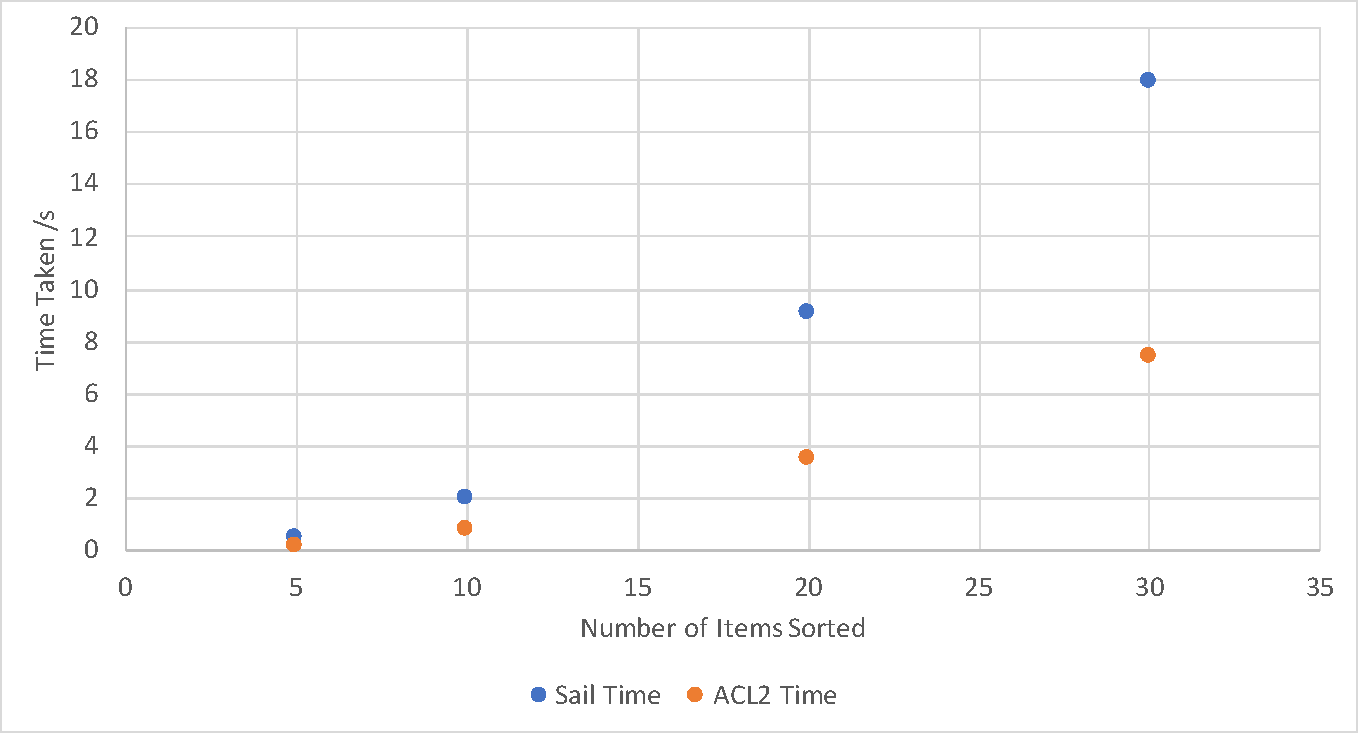
\includegraphics[width=\columnwidth]{../diagrams/speed.pdf}

\caption{Comparison of Sail and ACL2 Execution Times for Bubble Sort of Varying Input Size}
\label{diagram-speed}
\end{figure}

Figure~\ref{diagram-speed} shows the time in seconds for both emulators to complete a bubble sort of varying size.  The input to each program comprised a list of numbers in reverse order so the quadratic time is as expected.  The ACL2 emulator outperforms the Sail emulator by $2.6 \pm 0.2$ times.

This result is unsurprising.  The underlying Lisp implementation, SBCL, is heavily optimised for arbitrary precision integer arithmetic and Goel emphasises the optimisations she makes to the x86 ISA model itself throughout her paper~\cite{goel-thesis}.  Sail, on the other hand, is better suited to fixed precision bitvector manipulation---the first obvious optimisation would therefore be to infer such bitvector widths in the translated model.

Other optimisations include: implementing more functionality manually at a higher level (at the expense of less automation) to reduce call stack depth; and tightening up static typing as mentioned in Section~\ref{type-approx} to reduce the number of dynamic type checks.


\section{Conclusion---Results}

This chapter has presented the co-simulation technique and shown how it flagged up an implementation error in the original ACL2 model.  It has described how the coverage provided by the test suite is not ideal---this situation could be improved by using an instruction generator which creates instructions based on the code or structure of x86-64 instructions.  It has also shown some of the main features of the translator and how the implementation details described in Chapter~\ref{chapter-method} influenced them as well as undertaking an example performance comparison.

\hypertarget{chapter-related}{
\chapter{Related Work}\label{chapter-related}}

In normal compilation, the features of a high level language are progressively encoded in lower level representations until machine code is generated.  Source-to-source compilation refers to the translation of one language to another whilst retaining a similar level of abstraction.  This section covers examples of work in this area, related both to ISA models and to using Lisp as the source language, and compares them with the scenario this paper addresses.

\hypertarget{sail-as-target}{
\section{Using Sail as the Target Language}\label{sail-as-target}}

As part of the development of Sail, Armstrong et al.~\cite{sail-paper} developed a tool to automatically translate Arm's ASL into Sail.  One difficulty was type translation, although both ASL and Sail are first order imperative languages with static light-weight dependent type systems making them not too far removed.  Much of the complexity in converting ACL2 to Sail came from the much larger gap in type systems: the necessity to robustly infer types statically using disparate information spread throughout the ACL2 code.  One advantage for the ASL converter was that it was developed alongside Sail: features of the former steering the design of the latter (for example exception support and arbitrary precision rationals).  Although changes were made to the Sail codebase during this project, they were limited to minor modifications such as improving error messages or adding small utility functions, rather than language design.  In any case, the similarity of ASL and Sail make this co-design appropriate, whereas in general, the broader scope of ACL2 makes it less applicable, although fortunately many stylistic features of the x86 model itself made it amenable to translation to Sail.

\section{Using Lisp and ACL2 as Source Languages}

In general, Lisp is known as the go-to language for metaprogramming, however this often refers to its ability to define domain-specific languages and convert them into Lisp code, rather than translating Lisp code to other languages.  Despite this, there are cases where Lisp is used as the input language in source-to-source compilers.

\begin{sloppypar}
Perhaps the most well-known is ClojureScript, as described by McGranaghan~\cite{background-clojure-script}, which is of interest because it compiles, not to a lower-level language, but to JavaScript.  The most relevant comparison to our project is its handling of macros.  Macros are fully expanded at compile time and the resulting code is then compiled into JavaScript~\cite{background-clojure-script-macros}.  Overall, however, many details are less similar: JavaScript is dynamically and weakly typed, unlike Sail which is strongly and statically typed, making JavaScript an easier target than Sail; one focus of ClojureScript compilation is size of output code, which is not a concern in this project; conversely, human-readability of the output code is important in Sail, but less so for the ClojureScript compiler.
\end{sloppypar}

The most relevant example comes from Mark Staples~\cite{staples} who designed a framework for creating a shallow embedding of ACL2 in HOL.  Many techniques he used are similar to ones used in this project, such as:

\begin{itemize}
  \item Expanding macros before translation.
  \item Providing a set of translations for basic Lisp forms (such as literals and arithmetic expressions) whilst allowing more complex forms to be translated using either pattern matching (shown below) or via arbitrary translations.
  \item Developing some \emph{type guessing} heuristics to translate untyped lists into typed HOL terms.
  \item The assumption of monomorphism.
  \item The acknowledgement that \texttt{nil} is tricky to translate.
\end{itemize}

To demonstrate the framework he presented the translation of ACL2's \emph{Small Machine} theory---a model of a toy computational machine.  The example uses simple patterns to translate ACL2 expressions.  For instance, \texttt{("(EQUAL X Y)" , 'X == Y', [])} specifies that the Lisp list beginning with \texttt{EQUAL} should be translated to the infix term \texttt{==} with recursively translated sub-expressions \texttt{X} and \texttt{Y}.  Typing is directed from the HOL end: in this example, the use of \texttt{==} means that a function with a boolean return type is produced.  Human-directed type guessing is used to infer the types for \texttt{X} and \texttt{Y}: they can be specified as either naturals or integers.  It is also used to inform the translation of \texttt{nil}.

There are some notable differences between Staples' approach and this project.

\begin{itemize}
  \item Type information in the ACL2 syntax is not used.  Although the type guessing framework is extensible it is not clear that it would be as versatile as the solution in this project.
  \item Staples' approach is designed for dynamic translation between two running instances of ACL2 and HOL.  This project implements a static translation, which Staples noted would likely not be fully automatic.
  \item Staples notes that it is sometimes sensible to translate an ACL2 definition as a constant in HOL (where there is neither a handwritten nor automatic implementation) and only fully translate theorems about it.  Our translation to Sail was required to be executable, so this technique is not applicable.
  \item Staples focusses on creating the overall translation framework, leaving scope for individual projects to implement their own translations with term and type guessing extensibility.  This project effectively implements those details for the ACL2 x86 model.
  \item The Small Machine example was limited and did not cover many of the complexities encountered in this project.
\end{itemize}

There is, however, a project from Susanto and Melham~\cite{AMBA} which made use of Staples' tool by integrating a formal model of an ARM7 core written in Lisp/ACL2 with formal reasoning techniques in HOL.  The function which modelled execution in ACL2, \texttt{ARM7execute} was used as a base-constant in HOL, and ACL2 was treated as an \emph{axiom-server} to provide theorems about it.  This demonstrates that Staples' translation tool was sophisticated enough to be used in a large project but shows how its dynamic nature allowed less to be translated than is required in this project.

Another paper based on Staples work from Michael Gordon et al.~\cite{gordon} creates a deep embedding where Lisp lists (s-expressions) are represented directly in HOL and only built-in, undefined functions are translated by hand.  This increases confidence in translated theories compared with Staples' approach because the translation to the s-expression representation in HOL is relatively simple and, from there, properties about s-expressions (and then the translated definitions) are formally verified in HOL.  In other words, a model of Lisp is created within HOL.  This approach is suitable for formal reasoning but not for translation into Sail: we want both efficient execution and an idiomatic code style.


\section{Conclusion---Related Work}

This chapter has identified the related work in translating both from Lisp/ACL2 and into Sail.

\hypertarget{chapter-conclusion}{
\chapter{Conclusion}\label{chapter-conclusion}}

This dissertation has presented a translation into Sail of a model of the x86 ISA.  The main contributions can be categorised into two themes:

\begin{enumerate}
  \item \textbf{The Translator}.  Translating from ACL2 into Sail was a non-trivial task for the following reasons: ACL2 is dynamically typed but Sail is strongly and statically typed; there were ambiguities caused by ACL2 terms such as \texttt{nil}; and there were a large number of ACL2 tokens which needed intricate, manual translations to produce idiomatic Sail code.  Algorithms and heuristics were developed to resolve ambiguities and unknown types.  A trade-off between Sail code style, translator maintainability and translator automation was noted.

  \item \textbf{The Translation}.  Co-simulation was used to validate the Sail translation against the original ACL2 and an error in the original ACL2 model was discovered.  Coverage analysis of the chosen external test suite showed where coverage could be improved.
\end{enumerate}


To conclude, Greenspun's satirical \emph{tenth rule}~\cite{greenspun} states ``\emph{Any sufficiently complicated \ldots program contains an \ldots implementation of half of Common Lisp}''.  Although this hints that many Lisp features are desirable in other languages this is not universally the case, and it is hoped that translation into idiomatic Sail is one case where such a `half implementation' is justified.

\appendix
\singlespacing

% \bibliographystyle{unsrt} 
\phantomsection
\clearpage
\addcontentsline{toc}{chapter}{Bibliography}
\bibliography{refs.bib}

\end{document}
